\documentclass{pnastwo}


\usepackage{graphicx}
\usepackage{epsfig,subfigure}
%\usepackage{PNAStwoF}
\usepackage{amssymb,amsfonts,amsmath}


\contributor{Submitted to Proceedings
of the National Academy of Sciences of the United States of America}
\url{www.pnas.org/cgi/doi/10.1073/pnas.0709640104}
\copyrightyear{2008}
\issuedate{Issue Date}
\volume{Volume}
\issuenumber{Issue Number}


\begin{document}

\title{Producing temporal anticorrelations using spatial information}

 \author{Landa E\affil{1}{Instituto de Ciencias Nucleares, Universidad Nacional Aut\'{o}noma de M\'{e}xico, 04510 M\'{e}xico, D.F., M\'exico.},
 Irving O. Morales\affil{1}{}, \and Alejandro Frank\affil{1}{}\affil{2}{Centro de Ciencias de la Complejidad,
Universidad Nacional Aut\'{o}noma de M\'{e}xico, 04510 M\'{e}xico, D.F., M\'exico.}}

\contributor{Submitted to Proceedings of the National Academy of Sciences
of the United States of America}

\maketitle

\begin{article}

\begin{abstract} 
In this work we present a proposal to introduce temporal anticorrelations based on spatial information in contrast to those reported in the literature which involve measuring the arrival events emitted at random times in accordance with a homogeneous poisson point process where subsequently a deletion process with a predetermined time is applied, the proposed method is based with an entirely different paradigm. Both approaches are discussed and tested with analytical tools in order to stress the advantages of each one.
\end{abstract}

\keywords{Time Series | Correlations | Information}

%\abbreviations{}
%\abbreviations{SAM, self-assembled monolayer; OTS, octadecyltrichlorosilane}

\dropcap{M}any systems in nature can be in two or more stable states, obviously a stable state is a strong simplification, as internally generated dynamics and environmental stochasticity always cause fluctuations. Some of them can be driven by an external force out of equilibrium into a critical state which indicates a highly correlated or anticorrelated system~\cite{Schefer}. An extensively studied system with this behavior was introduced in physics, and is known as the Ising model in 2 dimensions, which is a model of a magnet at the microscopic level. The overall behavior of the system will vary depending on the temperature which determines when the system can undergo a phase transition between two different states, the ferromagnetic and paramagnetic phase. Many dynamical systems in different fields, including organism, financial markets, lakes, show a similar kind of behavior. Recent studies of tipping points (critical states) have shown that is notoriously difficult to predict when a system can shift abruptly from one state to another. Notwithstanding one of the most important generic indicators is to evaluate how strongly correlated (or anti-correlated) are the fluctuations, both spatially and temporally may indicate for a wide class of systems if a critical threshold is approaching~\cite{Dakos}. Returning to the above examples, one way to measure the intensity of the correlations (anticorrelations) is through the scale invariance property, {\it i.e.}, the exact or statistical independence of a system on the law that describes it on a chosen scale~\cite{Landa}. The lack of a characteristic scale is reflected in the strong correlation among different parts of the system, either on the spatial domain as a particular distribution of the size of clusters spread over many magnitudes, or on the temporal domain as a time pattern that can be found on many time scales. In this paper we use the traditional approach of time series analysis as a tool to analyze under what conditions is possible to get a highly correlated or anticorrelated time series which in turn describe the dynamics.  In this paper we use the traditional approach of time series analysis as a tool to analyze under what conditions is possible to get a highly correlated or anticorrelated time series which in turn describe the dynamics. We focus in the main characteristic scales which govern the anticorrelations in order to make evident the dynamical processes that are being generated internally in the systems, this approach could provide clues for the understanding more complex systems. In order to tackle the problem, two simple models based on certain rules to introduce anticorrelations are posed (see below). As a first step we concentrate on the statistical properties of the time series which are reflected in the random process governing the occurrence of events. If the events occur at perfectly regular times intervals has lower event-number fluctuations than temporal processes whose events arrive at statistically independent times. In the former case the number of events counted in any time $T$ is fixed, so that the second moment of the distribution $\sigma_{n} = 0$, whereas in the latter case a number of counts in any prescribed time interval obey the Poisson distribution, $\sigma_{n} = <n>$ for all $T$. Events-number fluctuations lower than those given by Poisson distribution (sub-Poisson) are possible in many context of science as well as event-number fluctuations upper than those given by Poisson distribution (super-Poisson). We concentrate in the fact that the events can be correlated or anticorrelated with previous events within different time scales, to prove the previous statement we calculate the normalized rate of event coincidences at two times separated by an interval $\tau$ (see below the mathematical formulation) which determines the degree and range of the correlations or anticorrelations. The normailized coincidence is equal 1 for all time delays $\tau$, if  the temporal events are associated with poisson point processes because arrive independently. However, if the normalized rate is less than unity indicates that the pairs of events delayed for a time $\tau$ are less likely to occur and therefore the occurrences are anticorrelated, this special feature is known as the property of anti-bunching. Otherwise, if the normalized rate is greater than unity, the opposite occurs and a bunching property is observed which is the tendency of events to distribute themselves preferentially in bunches rather than at random, antibunching is the opposite effect, in which fewer event pairs are detected close together than further apart. An important  note is that the poisson point process serves as the boundary between the time series with correlated events and those where events have the property to be anticorrelated. Therefore, we use poisson point process as a reference to subsequently implement various techniques in order to produce anticorrelations. We illustrate the statistical properties mentioned above to quantify the inherent properties of the time series produced with our models, the standard measures mentioned above have been widely used in the quantum theory of light. The main aim is to understand how produce the long time anticorrelations (correlations) in an uncorrelated simple process, our models stresses the significant memory effects in the system to cause such kind of anticorrelations. These analysis can provide a simple understanding of the description of anticorrelated processes in complex systems. It involves in details how a feedback mechanism implicated in our simulations for the annihilation of events generates a dynamical state with long range anticorrelations.



\section{Modelling the Poisson point processes}
\label{model}

A brief discussion about a poisson point process is exposed. A random point process is a countable set of random points located on the real line. The basic example of such process is the Poisson process, since it is one of the most important point processes which plays an equivalent role to the normal distribution within the statistical distributions. A point process $\{ t_n : n \ge 0 \}$ on the positive line, is a Poisson process of intensity $\lambda>0 $ if it satisfies the following conditions: (i) The process has independent increments for each finite collection of times, $0 = t_0 <t_1 <\cdots <t_n$, and also the increments $N(t_ {i-1}, t_ {i}] = N (t_i)-N (t_ {i-1}) $, $ i = 1, \cdots, n $, are independent, and (ii) the individual increments N (s, t] = N (t)-N(s) have the Poisson distribution. The second condition can be decomposed into two parts; (a) temporal increments are homogeneous (i.e., the distribution of increments depends only on the length of the time interval but not of their position) and (b) the distribution of each individual increment is also a Poisson distribution, with a mean proportional to the amount of time considered. Have a temporarily homogeneous point process with independent increments means that if the process is restarted from any point in time $t$, the process thus obtained is independent of what happened earlier (by having independent increments) and has the same distribution as the original process (by being temporarily homogeneous). In other words, the process has no memory. We generate poisson point processes using the NetLogo platform~\cite{Netlogo} that allows to carry out numerical experiments. In what follows, we have taken the analogy between a process of events that follow a Poisson distribution with a gun that shoots a stream of bullets at random~\cite{Teich}. Schematically in Fig.~\ref{fig1} can be appreciated the Poisson point process generated in the NetLogo platform through a snapshot of the simulation. The green block represents the hypothetical Poisson gun and the yellow circles the bullets fired in previous times, one important constraint of the model is associated with projectiles which move a constant speed during the simulation. The arrivals of the projectiles at $t_n$ are detected by the red block (which represents the detector). The events $t_n=\sum_{i=1}^{n}T_i, \,\, n=1,2,\ldots$ with $t_0=0$  are generated using a sequence of positive random variables and independent, each one obtained from an exponential distribution with intensity $\lambda$. The arrival process $\{ t_n : n \ge 0 \}$ is a Poisson point process  with intensity $\lambda$ according to the condition (ii). An example of this type of process in nature has been extensively studied in quantum optics and is based on the behavior of light (the distribution of photons) produced by a laser~\cite{Teich}. In order to understand the systematic way of how temporal anticorrelations are introduced in a simple system, we explore via the modification of the process. Essentially following the analogy of the hypothetical gun mentioned above the production of antibunched point process can be achieved in three ways: by regulating the times at which the trigger is pulled, by introducing constraints into the firing mechanism, and/or by selectively deleting some of the Poisson bullets after they are fired, each of these techniques involves the introduction of anticorrelations which results in a small predictable number of events. In the next section some methodologies which are discussed extensively in the literature to introduce anticorrelations into a Poisson point process are disclosed.  


\section{Methodologies to introduce anticorrelations}
\label{methodologies}

The discussion below is essentially confined to those control rules to convert random emission events in emissions whose temporal fluctuations obey a sub-Poisson distribution, some of them are illustrated in Fig.~\ref{fig2}. It is assumed for simplicity that the conversion can be achieved in an ideal form. We stress that all methods described below are discussed in a quite general context, i.e., the agents in the numerical simulation under certain circumstances may represent different entities, which it means they can be applied to a wide range of situations. In our context, the direct generation of the time series that represent Poisson point processes may be visualized in terms of ball sequences which are randomly shot from the hypothetical gun. At the moment that the balls emerge from the gun, they do with a Poisson number distribution and just then a specific mechanism is implemented to regularize the stream in order to introduce anticorrelations which results in a more regular flow of events, exhibiting a sub-Poisson behavior in the temporal fluctuations. In the next lines are presented some techniques used in the literature~\cite{Teich1}. {\it Dead-Time Deletion}, one may make the sequence more regular by deleting every event that follows another within a prescribed fixed dead time $\tau_{d}$, i.e., the dead-time prohibits a second event from occurring within a fixed time following the occurrence of a given event. Therefore it prevents the events from being arbitrarily close to each other by decreasing the randomness of the number of events registered in the fixed counting time $T$, as is shown in Fig.~\ref{fig2} (b). {\it Coincidence Decimation} is a process which closely spaced pairs of events are removed if they are separated by a time shorter than a prescribed time interval $\tau_{cd}$. This procedure is shown in Fig.~\ref{fig2} (c). {\it Decimation} is a process that selects every $n$-th event ($n=2,3,�$) of an initially Poisson point process, deleting all intermediate events. The passage of every other event ($n=2$) is explicitly illustrated in Fig.~\ref{fig2} (d), the regularization effect on the event stream is similar to that imposed by dead-time deletion. There are at least two more ways not treated here to produce anticorrelated and sub-Poisson behavior amply discussed in the two previous references, both mainly deal with the same idea to regulate the interval times between the events. We quantify the intensity and range of the introduced anticorrelations, we focus mainly in the coincidence rate between events and the statistics of the number of counts in prescribed intervals to measure the dispersion on the processes, both quantities are quite standard in classical and quantum theory of light, for simplicity are explained in that framework. The semiclassical theory of light treats the radiation field classically while using the quantum theory to describe the interaction of the light with the atoms of the detector. Light is represented by means of a random complex analytical signal $V(\mathbf{x})$ (where $\mathbf{x}$ is the space-time point ($\mathbf{r}$,t)), whose squared absolute value $I(\mathbf{x})$ is the optical intensity. Light fluctuations are completely characterized by the statistic of the stochastic process $V(\mathbf{x})$. At a space-time point $\mathbf{x}$ the most important descriptor is the probability density $P(I(\mathbf{x}))$ of the intensity, its mean $<I(\mathbf{x})>$, and its variance $Var(I(\mathbf{x}))$. Fluctuations at two space-time points $\mathbf{x}_1$ and $\mathbf{x}_2$ can be characterized by the intensity correlation function (also called second-order correlation function)
\begin{equation}
G^{(2)}(\mathbf{x}_1,\mathbf{x}_2)=<I(\mathbf{x}_1)I(\mathbf{x}_2)>,
\label{eq2}
\end{equation}
as well as its normalized version
\begin{equation}
g^{(2)}(\mathbf{x}_1,\mathbf{x}_2)=G^{(2)}(\mathbf{x}_1,\mathbf{x}_2)/[<I(\mathbf{x}_1)><I(\mathbf{x}_2)>].
\label{eq4}
\end{equation}
This quantity is also known as the degree of second-order coherence. When light is detected by a photodetector such as a photomultiplier tube, the photoelectron arrivals at different locations and times are describable by a doubly stochastic Poisson point process (DSPP), whose rate is the stochastic function $\eta I(\mathbf{x})$, where $\eta$ is the quantum efficiency of the detector. The probability of coincidence of two photoevents within incremental areas $\Delta A$ and time intervals $\Delta T$, surrounding the space-time points $\mathbf{x}_1$ and $\mathbf{x}_2$, is given by $\eta^{2} G^{(2)}(\mathbf{x}_1,\mathbf{x}_2)(\Delta A\Delta T)^{2}$. The normalized intensity correlation function $g^{(2)}(\mathbf{x}_1,\mathbf{x}_2)$ therefore represents the join probability of occurrence of one photoevent detected $\mathbf{x}_1$ and another at $\mathbf{x}_2$, normalized by the product of the marginal probabilities that a photoevent occurs at $\mathbf{x}_1$ and that a photoevent occurs at $\mathbf{x}_2$. According to previous definition, light characterized by a deterministic intensity $I(\mathbf{x})$, and by degrees of coherence whose absolute values is unity, signifying that the join probability of coincidence of a photoevent at $\mathbf{x}_1$ and another at $\mathbf{x}_2$ equals the product of the marginal probabilities of an event at each point, that is, photoevents occur independently or in total randomness, is called coherent light. If $g^{(2)}(\mathbf{x}_1,\mathbf{x}_2)>1$, the occurrences of events at the two points are positively correlated, that is, when one occurs, the other is more likely to occur (bunched). Alternatively, when $g^{(2)}(\mathbf{x}_1,\mathbf{x}_2)<1$, photoevents are anticorrelated, that is, when one occurs, the others is less likely to occur (antibunched). In the limit when the two space-time points are very close to each other, that is, when $\mathbf{x}_{1} \sim \mathbf{x}_{2} = \mathbf{x}$, the normalized coincidence rate is measured by the function $g^{(2)}(\mathbf{x},\mathbf{x})$, particularly that which we measure in our simulations because of the experimental setup used. We also apply the Fano {\it factor} that is an important descriptor of photocount statistics and is the ratio between the variance and the mean of photocounts $n$~\cite{Fano}.
\begin{equation}
F_{n}(\mathbf{\ell})=\frac{Var(n)}{<n>}.
\label{eq6}
\end{equation} 
The Fano factor depends on the length counting box over the time series (represented by $\mathbf{\ell}$). For coherent light $n$ is Poisson distributed and $F_{n}(\mathbf{\ell})$=1, independent of $\mathbf{\ell}$. Light for which $F_{n}(\mathbf{\ell})>1$ is said to exhibit super-Poisson behavior in the domain $\mathbf{\ell}$ in which this inequality is obeyed. Such light suffers from fluctuations larger than those of the Poisson. When $F_{n}(\mathbf{\ell})<1$, the photocounts are said to exhibit sub-Poisson behavior. The second-order correlation function and the Fano factor according to the quantum theory of light is implemented to those time series obtained with the NetLogo platform, these measures serve as a reference frame to perceive what type of correlations have been introduced. As a last measure we extend quite a lot the application of the Fourier basis to calculate the power spectrum directly to the time series, this analysis allows to know the structure of the decay of the correlations using the Wienner-Khinchin theorem which stablishes that the power spectral density of a random process is the Fourier transform of the corresponding autocorrelation function. In order to illustrate the measures explained above an analysis based on numerical simulations is exposed in this section. The first numerical experiment consists of three ensembles with 100 realizations each one, all of them obtained by dead-time deletion control with $\tau_{d}$ equal to 2, 10 and 50. The Poisson point process generated initially is characterized by obeying a exponential distribution with average 5 for all cases. The corresponding $g^{2}(\tau)$ functions are shown in the Fig.~\ref{fig3}, it can be seen very clearly how the coherence is totally destroyed within the $\tau_{d}$ duration, this is represented by a flat region where the $g^{2}(\tau)$ takes the value 0. Afterwards of the prescribed dead time value a increase value in the coincidence rate is observed, this is a consequence of the most likely value for an occurrence during the simulation processes which is precisely the immediate value to $\tau_{d}$, {\it i.e.}, there is higher probability to measure events immediately after $\tau_{d}$ and periodic values of it, this is very noticeable for $\tau_{d}=50$. The ratio between variance and mean derived as an average are 0.11, 0.019 and 0.02, respectively. Despite the fact that Fano factor is lower than 1 these methods are not suitable to introduce long-range anticorrelations in all temporal scales. Another important aspect is that the anticorrelations in scales smaller than the fixed dead times are nulls because of the restriction of the $\tau$ value. The power spectra analysis shows periodicities due to the existing fluctuations around the most likely event imposed by the dead times in the time series generated, a significant power law relationship is not found to each case, see Fig.~\ref{fig4}. Equivalent results are obtained for coincidence decimation and decimation method, therefore the analysis has been omitted. So far, the discussed methods produce nulls anticorrelations between the events of a given length by the fixed dead time or a prescribed time interval, anticorrelations are not properly generated even though $g^{2}(\tau) < 1$ for certain values of $\tau$. In view of the obtained results we present in the following section a new proposal to introduce anticorrelations at different time scales.

\section{Proposal I}
\label{proposal1}

A schematic picture of the previous simulations in terms of the emission probability for each projectile is presented in Fig.~\ref{fig5}. The emission probability is zero until the dead time takes the value $\tau_d$ where the probability takes the maximum value. The new proposal in this section is based on a method which is not restrictive in the selection of the dead time value due to it can be taken of a certain range [$ 0, \tilde{\tau}_ {e}$], this idea is based only in a simple modification of the dead time control. We use an exponential probability function ($e^{\gamma \tilde{\tau}_{e}}$) as it is shown in Fig.~\ref{fig5} (thin dotted line), which is explicitly determined by a single parameter label, $\gamma$. The values of the parameter $\gamma$ in the numerical simulation are 0.0010, 0.0015, 0.0030 and 0.0045. The functions $g^{2}(\tau)$ for each case of $\gamma$ are shown in Fig.~\ref{fig6} (a), the behaviors are quite different from the cases discussed above, the major difference is that the functions $g^{2}(\tau)$ decay smoothly to zero which implies that there are anticorrelations at different scales within the range allowed and fixed by $\tilde{\tau}_ {e}$. Time series generated with this method have an associated Fano factor less than unity and a power spectrum with a shape shown in Fig.~\ref{fig6} (b), clearly there is a difference with the power spectra obtained in the previous section, the difference is a linear trend for a specific range in the frequency domain. The proposed method greatly improves the introduction of anticorrelations between the events in the uncorrelated time series generated initially by the hypothetical gun. Importantly, the method allows immediate anticorrelation between events, i.e., just between the nearest-neighbor events. Therefore, there is not information beyond the nearest neighbours. In the next section we propose a new method to control the intensity and length of the anticorrelations introduced in the time series starting from a different approach.

\section{Proposal II}
\label{proposal2}

In order to introduce long-range anticorrelations, the system should store information of the events in different time scales which in fact is a costly procedure. A paradigm shift is necessary to get long-range antcorrelations, the proposal in this section is based on considering a hypothetical material capable of storing spatial information of the events that have happened in previous steps. Therefore the removal procedure of events depends of how many events have occurred in previous steps of the simulation which is a quite different criterion compared with those mentioned in the previous sections. Essentially we simulate projectiles passing through a material which is partitioned into slices as can be seen in the upper panel of Fig.~\ref{fig7}. Each slice has the property to get excited every time that a projectile crosses it by an amount labeled as $\xi_{e}$. Coupled with the previous property there is another important peculiarity related to the material which is associated to a natural rate of relaxation labeled as  $\xi_{r}$, that acts throughout the whole simulation decreasing the degree of excitation. The medium has a peculiar property which gives the chance that the projectiles can split into a new pair of projectiles which move outside the straight path (they are schematically represented as red balls in upper panel of Fig.~\ref{fig7}), this fact allows to remove events in the time series which are measured using a detector at the end of the path (red rectangular block in Fig.~\ref{fig7}), this process plays an analogous role to deletion controls mentioned previously. To carry out the mentioned stochastic process is necessary to define a control parameter labeled as $\Lambda_{d}$, its role is basically analogous to a dice with faces equal to the value of $\Lambda_{d}$ and sets the probabilistic limit to determine whether the projectile can be split or not. There is an accumulated value associated to the excitation property labeled as $G_{\acute{x},t_i}(\xi_ {e})$ at the instant time $t_{i}$ and the position $\acute{x}$, i.e., $G_{\acute{x},t_i}(\xi_{e})=\sum_{t=1}^{t_{i}}\delta(x-\acute{x}) \xi_{e}$ which is a particular value of each slice and is given by the evolution of the simulation. Numerically at the beginning $G_{\acute{x},t_i}(\xi_ {e})$ takes the zero value. As time increases $G_{\acute{x},t_i}(\xi_ {e})$ grows by the amount associated to the parameter $\xi_{e}$, so that during the simulation each slice will have a specific value of $G_{\acute{x},t_i}(\xi_ {e})$. The above effect mentioned is reflected in the lower panel of the Fig.~\ref{fig7} where is possible to notice the intensity of the excitation level along horizontal axis. The $\Lambda_ {d}$ parameter together with $G_{\acute{x},t_i}(\xi_ {e})$ determine the ratio $P_p=G_{\acute{x},t_i}(\xi_ {e})/\Lambda_ {d}$ which defines whether the projectile splits or not. With $P_p$ bigger than 1 the projectile always splits in a new pair of projectiles that come out at an certain angle so they are not taken into account in the final time series but if $P_p <1$ the projectile continues its straight path to the next slice where the stochastic process is repeated again until the projectile reaches the detector or finally splits. The property of relaxation is fixed during the whole simulation with the aim of reducing the likelihood of conversion and allows that the projectiles can reach the detector position. The parameters $\xi_{e}$ and $\xi_{r}$ are modifying the properties of the medium, Figure~\ref{fig7} displays a static part of the simulation, it can be seen how the excitation property allows the splitting. $G_{\acute{x},t_i}(\xi_ {e})$ changes every time step for some slices inside the material playing a similar role of the dead time interval $\tau_{d}$ in the {\it exponential deletion} method. There is also a spatial information in the converted projectiles because is most likely being converted in the zones where $G_{\acute{x},t_i}(\xi_ {e})$ is higher. Both degrees of freedom generate anticorrelations on different time scales into the time series generated. In the numerical experiments the Poisson point process remains unchanged as in the previous sections and the length of the material is fixed, each slice corresponds a discrete unit time. Having thoroughly analyzed different combinations in the parameters, we present the results as follows. The ensembles consist of 50 realisations each one, the length of the time series are of 4 000 events. The first result follows the specific parameters shown in the Table~\ref{table1}. Figure~\ref{fig8} shows the functions $g^{2}(\tau)$ for each value of  $\Lambda_ {d}$ with the others parameters fixed. The intensity of the functions $g^{2}(\tau)$ decays with different slopes according to the magnitud of $\Lambda_ {d}$ and is smaller than 1 until $\tau \simeq 30$ where starts to fluctuate around 1, except for $\Lambda_ {d}$ equal 10000 where practically the autocorrelations correspond to Poisson processes which serves as a reference frame in our simulations. It is also evident as the autocorrelations decreases when $\Lambda_ {d}$ increases, for this case $\Lambda_ {d}$ can be used as a control parameter for the strength in the autocorrelations. For higher values of $\tau \simeq 60$ the value of $g^{2}(\tau)$ tends to one and no more anticorrelations between events are present. For values of $\Lambda_{d}$ equal to 50 and 100, the intensity of $g^{2}(\tau)$ is zero for $\tau \simeq 0$ and increases up 1 as $\tau$ takes bigger values, for the other values of $\Lambda_{d}$ the intensity of the function for $\tau \simeq 0$ is not zero which indicates a weaker anticorrelation between the events for $\tau$ values close to zero. For values of $\Lambda_{d}$ lower than 50, the normalized correlation function starts having a similar behavior to that obtained with dead time deletion. The magnitude of the fluctuations compared with those of Poisson distribution are appreciated in Table~\ref{table1}. The Fano factor as a function of $\Lambda_ {d}$ show a clear increasing trend, a contrary manner to the evolution of the values related to the exponents $\beta_{PS}$ obtained through the power spectrum which are shown in Fig.~\ref{fig9}. The fit  to the linear trend of the the power spectrum ($P(f) \sim f^{\beta_{\mathrm{ps}}}$) is obtained for all ensembles and is reported in Table~\ref{table1}. The value of the exponent $\beta_{\mathrm{ps}} $ is approximately equal to 1 for $\Lambda_ {d} = $ 50 and begins to decrease as $ \Lambda_ {d} $ increases, this can be seen in Fig.~\ref{fig9} where the power spectrum for $\Lambda_ {d} = $ 50 is plotted in the lowest part of the figure, the subsequent power spectra are plotted in the upward direction following the order given in Table~\ref{table1}. The lats power spectrum plotted is for $\Lambda_ {d} = $ 10,000 where the exponent $\beta_{\mathrm {ps}} $ obtained is almost 0 which corresponds a purely random signal. The second important result obtained is shown in Fig~\ref{fig10} and consists of ensembles with equal dimension as in the previous case. Now the parameters fixed are $\Lambda_{d} = 100$ and $\xi_{e} = 5$ and the only parameter changing is $\xi_ {r}$ which takes values from 0.1 to 0.5 in steps of 0.1 as is shown in the legend of the figure. The remarkable thing with this variant has to do with the time scale range in the introduced anticorrelations see Fig.~\ref {fig10} where the $g^{2}(\tau)$ functions are plotted. We are able to control the time scale of the anticorrelations between different events unlike previous methods which consist only with the neighbor events. The Fourier analysis is presented in Fig.~\ref{fig11}, where the power spectra have been displaced vertically to avoid an overlap of data. The power spectrum with the longest range anticorrelations is plotted in the lowest part of the figure and so on until the shorter range in the upper, clearly the power spectrum to each one is shifted horizontally in accordance with the increasing value of $\xi_{r}$, i.e, the linear part of the power spectrum takes another interval in the frequency domain to be precise at bigger frequencies than indicate shorter time scales. Comparing the results obtained with those shown in Fig.~\ref{fig9}, is remarkable how the frequency range is shifted horizontally in contrast to a change just in the spectral density. Also a linear regression is shown, the numerical value for $\beta_{\mathrm{ps}}$ is $0.66$ for each case (there are very small deviations in each one) because the shape of the spectrum does not change. A similar behavior for $g^{2}(\tau)$ and the power spectrum $P(f)$ is observed when the parameters $\Lambda_{d}$ and $\xi_{r}$ are kept fixed, this because the parameters $\xi_{r}$ and $\xi_{e}$ are linked because are not independent. 

   

\section{Conclusions }
\label{conclusionss}

We generate anticorrelated time series through different methods, some of them mentioned previously in literature. In the case of dead time deletion control the introduced anticorrelations are spurious and only cover the lag time given by $\tau_{d}$. Even though the fluctuations in the event count statistics are smaller than 1, which indicates sub-Poisson behavior the time series do not properly represent an anticorrelated process. Two different methods to introduce anticorrelations are proposed, the exponential time deletion which the $g^{2}(\tau)$ functions are more in accordance with those anticorrelated processes in nature, for instance the quantum light which is generated through an inhomogeneous nonlinear crystal which is pumped with a poisson process (laser) to generate anticorrelated photon time series. On the other hand, the last proposal to introduce long-range anticorrelations enables control the intensity and range of the introduced anticorrelations, the most important aspect of the latter model has been the importance of the spatial structure to store information which allows to create a memory effect in the system that helps to get correlated processes in different time scales, a simile in nature is in the flocking behavior which creates a coherent motion in time just with the spatial information between the neighbours of each element of the systems.

 
\begin{acknowledgments}
This work was supported in part by grants from CONACyT-Mexico and the project FP7-PEOPLE-2009-IRSES-247541-MATSIQEL. We are grateful to P. Str\'ansk\'y for his many suggestions.

\end{acknowledgments}



\begin{thebibliography}{}
\bibitem{Schefer} Scheffer M, Carpenter S R (2003) Catastrophic regime shifts in ecosystems: linking theory to observation. {\it Trends in Ecology and Evolution}, 18: 648-656.
\bibitem{Dakos} Dakos V, Carpenter S R, Brock W A, Ellison A M, Guttal V, Ives A R, K\'efi S, Livina V, Seekell D A, van Nes E H, Scheffer M (2012) Methods for Detecting Early Warnings of Critical Transitions in Time Series Illustrated Using Simulated Ecological Data. {\it Plos One} 7(7): e41010. 
\bibitem{Landa} Landa E, Morales I, Hern\'andez C, L\'opez Vieyra J C, Vel\'azquez V, Frank A (2008) Scale invariance and criticality in nuclear spectra. {\it Rev. Mex. Fis.},  S-54(2) 48.
\bibitem{Netlogo} Netlogo, http://ccl.northwestern.edu/netlogo/
\bibitem{Teich}  Teich M C and Saleh B E A (1982), Effects of random deletion and additive noise on bunched and antibunched photon-counting statistic. {\it Optics Letters}, Vol. 7 No. 8.
\bibitem{Teich1}  Teich M C and Saleh B E A (1988), I Photon Bunching and Antibunching. {\it Progress in optics, Elsevier}, 26.
\bibitem{Fano}  Fano U (1947), Ionization Yield of Radiations. II. The Fluctuations of the Number of Ions. {\it Physical  Review}, 72  26-29.


\end{thebibliography}

\end{article}

%%%%%%%%%%%%%%%%%%%%%%%%%%%%%%%%%%%%%%%%%%%%%%%%%%%%%%%%%%%%%%%%%%%%%%%%%%%%%%%%%%%%%%%%%%%%%%%%%%%%%%%%%%%

\begin{figure}[h]
\vspace {0.5 cm}
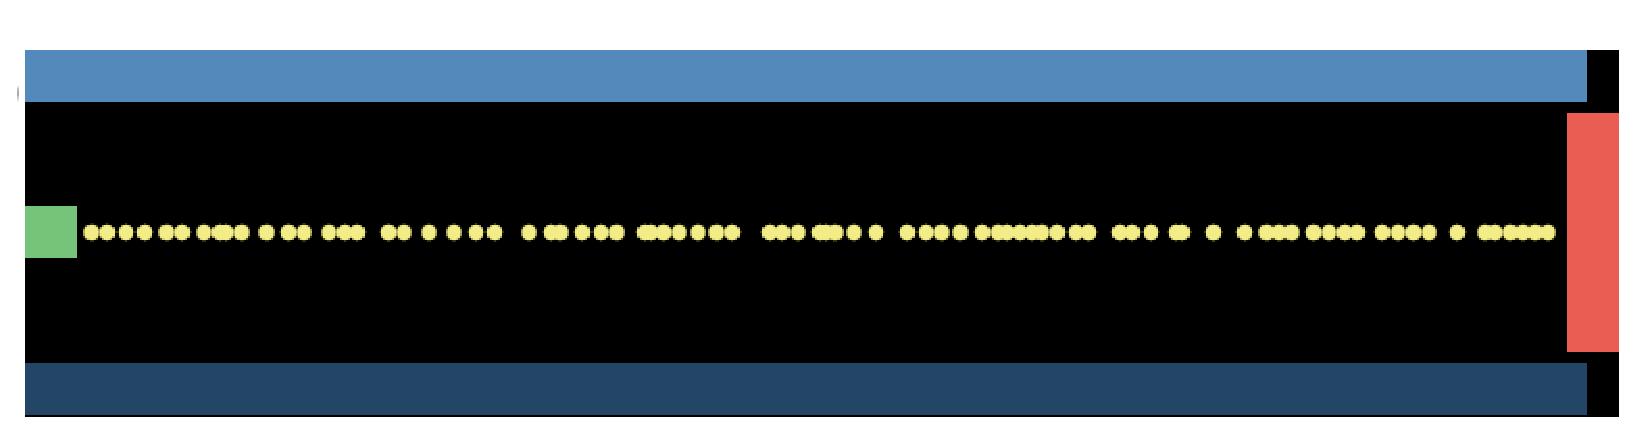
\includegraphics[width=\linewidth,angle=0]{figure1.eps}
\caption{Hypothetical poisson gun that is randomly fired to generate a stream of Poisson bullets that have a Poisson number distribution. The green block represents the hypothetical Poisson gun and the yellow circles the bullets fired in previous times. The red block represents the detector. A snapshot of the simulation with the NetLogo platform.}  
\label{fig1}
\end{figure}

\begin{figure}[h]
\vspace {0.5 cm}
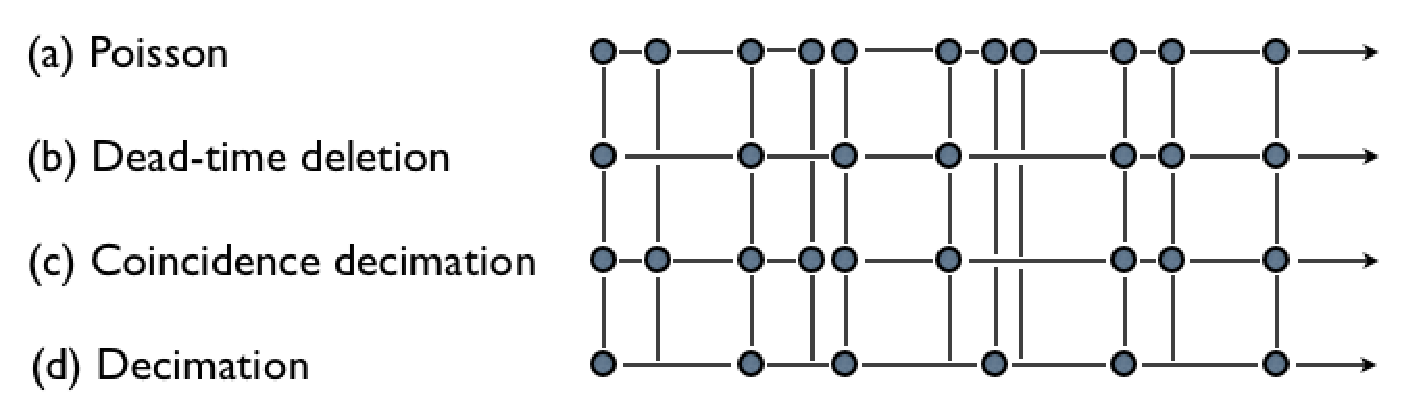
\includegraphics[width=\linewidth,angle=0]{figure2.eps}
\caption{Poisson point process is generated with the hypothetical gun (a). Anticorrelations can be imparted by any of three processes: The initial excitation process (trigger); the emission process (firing mechanism); or a feedback process derived from the emitted bullets that controls either of the other two processes. The stream become sub-Poisson (bottom rows of Poisson process) and antibunched process from (b) dead-time deletion, (c) coincidence decimation and (d) decimation.}  
\label{fig2}
\end{figure}

\begin{figure}[h]
\vspace {0.5 cm}
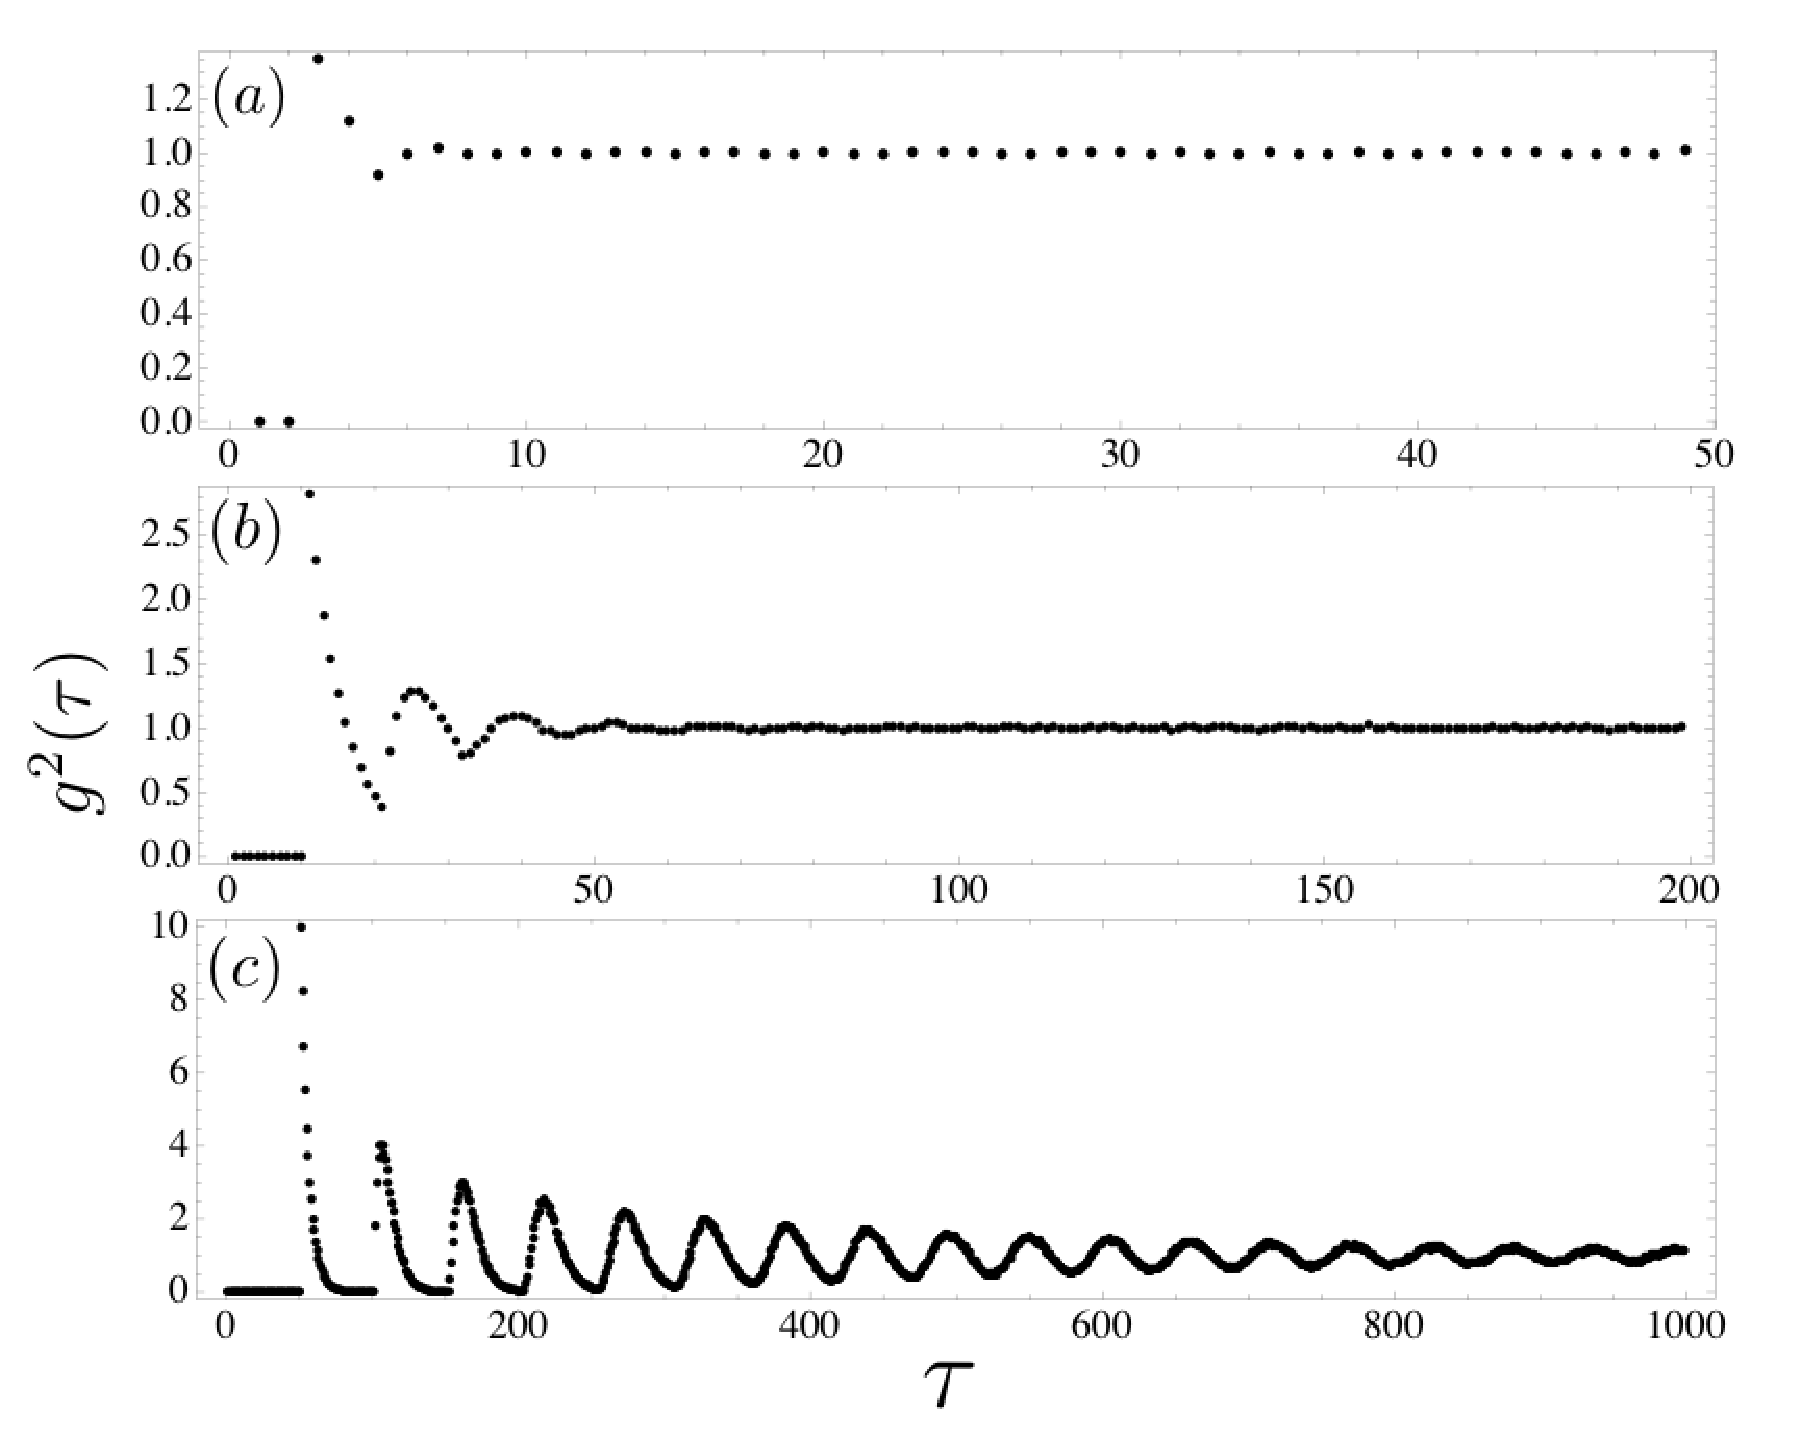
\includegraphics[width=\linewidth,angle=0]{figure3.eps}
\caption{$g^{2}(\tau)$ as a function of lag time values $\tau$ to quantify the coincidence rate for the time series obtained through dead-time deletion control. (a) $g^{2}(\tau)$ for a time series obtained within a fixed dead time $\tau_{d}$ equal to 2, (b) $g^{2}(\tau)$ for a time series obtained within a fixed dead time $\tau_{d}$ equal to 10, (c) $g^{2}(\tau)$ for a time series obtained within a fixed dead time $\tau_{d}$ equal to 50.}  
\label{fig3}
\end{figure}

\begin{figure}[h]
\vspace {0.5 cm}
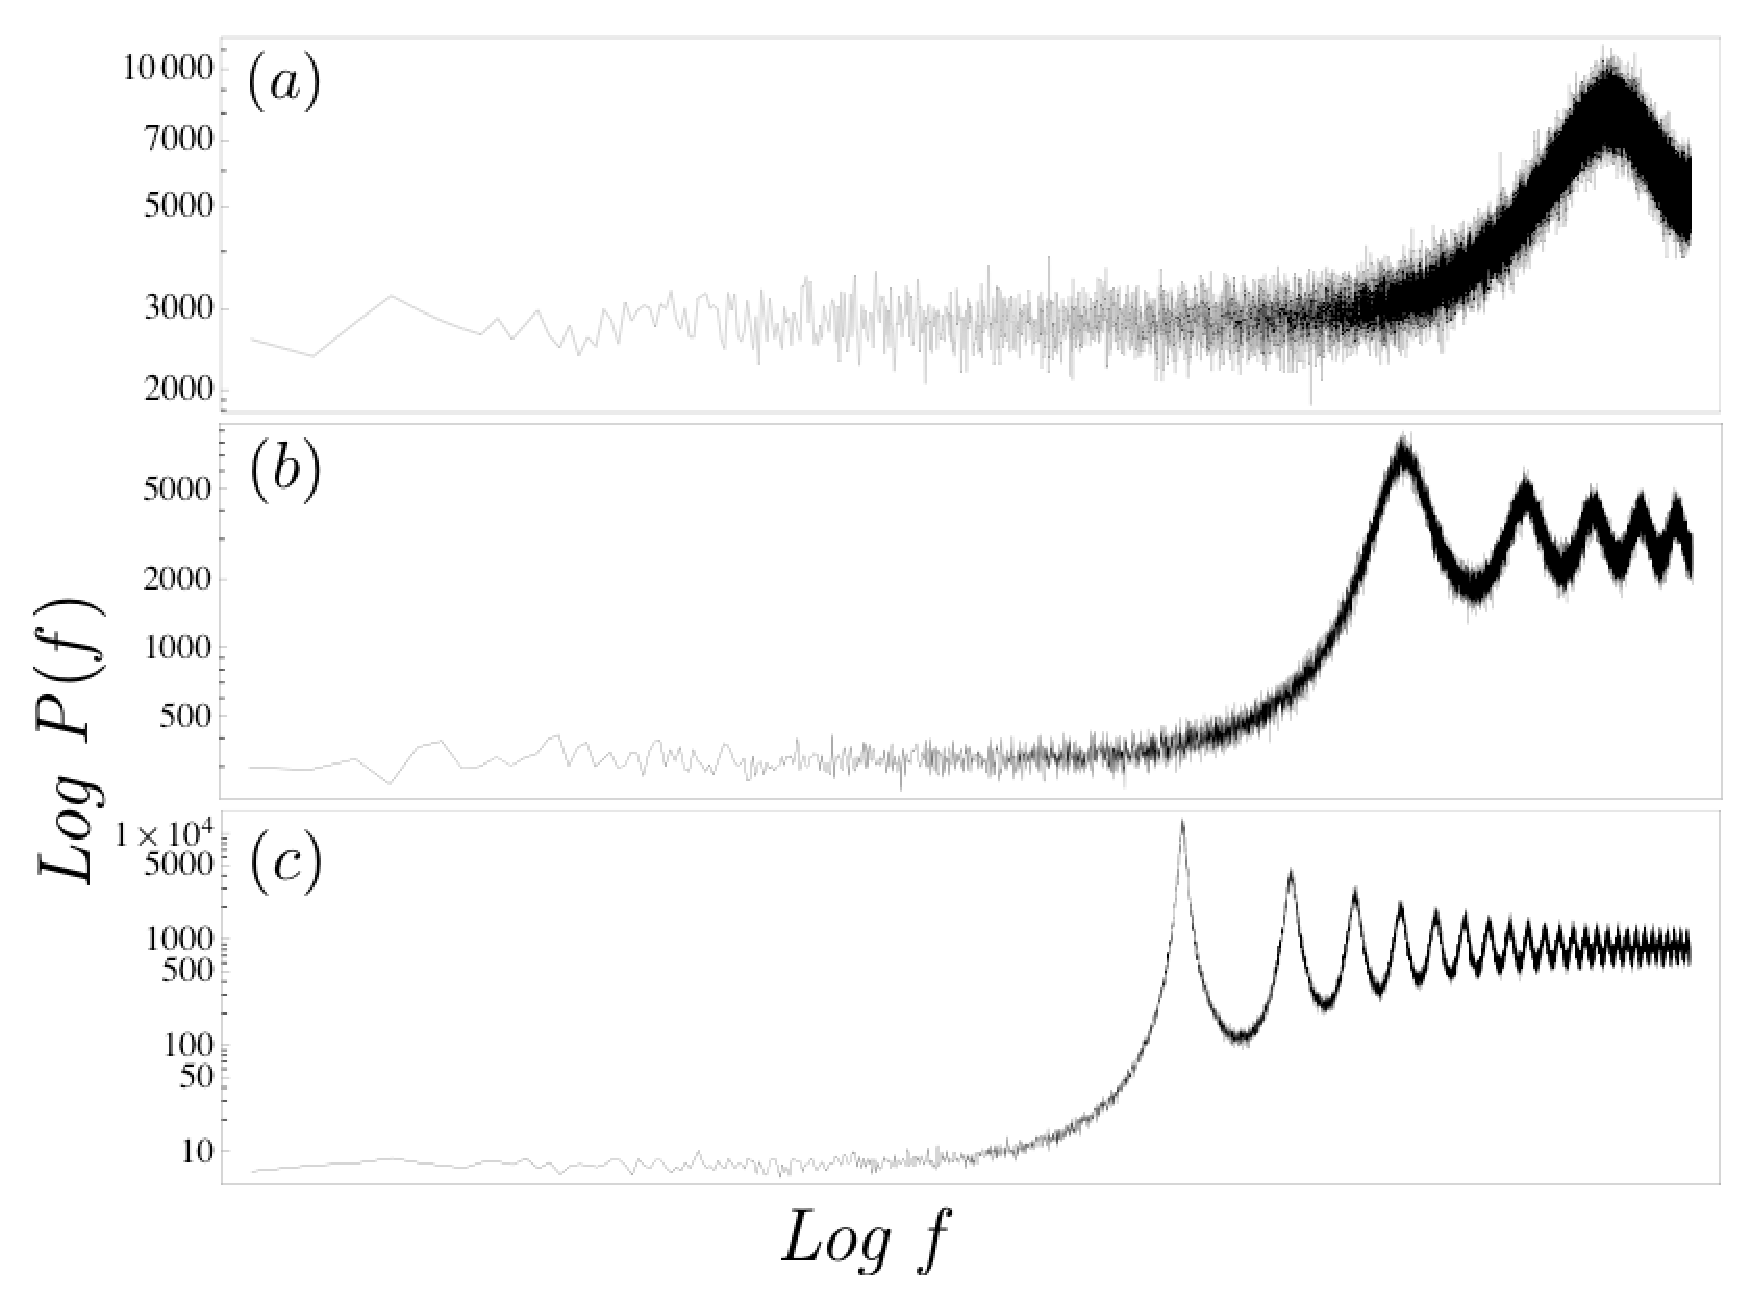
\includegraphics[width=\linewidth,angle=0]{figure4.eps}
\caption{Power spectrum $P(f)$ of (a) $g^{2}(\tau)$ for a time series obtained within a fixed dead time $\tau_{d}$ equal to 2, (b) $g^{2}(\tau)$ for a time series obtained with $\tau_{d}$ equal to 10, (c) $g^{2}(\tau)$ for a time series obtained with a $\tau_{d}$ equal to 50, and (d) $P(f)$ obtained from a time series generated with exponential time deletion with $\gamma =0.0030$.}  
\label{fig4}
\end{figure}

\begin{figure}[h]
\vspace {0.5 cm}
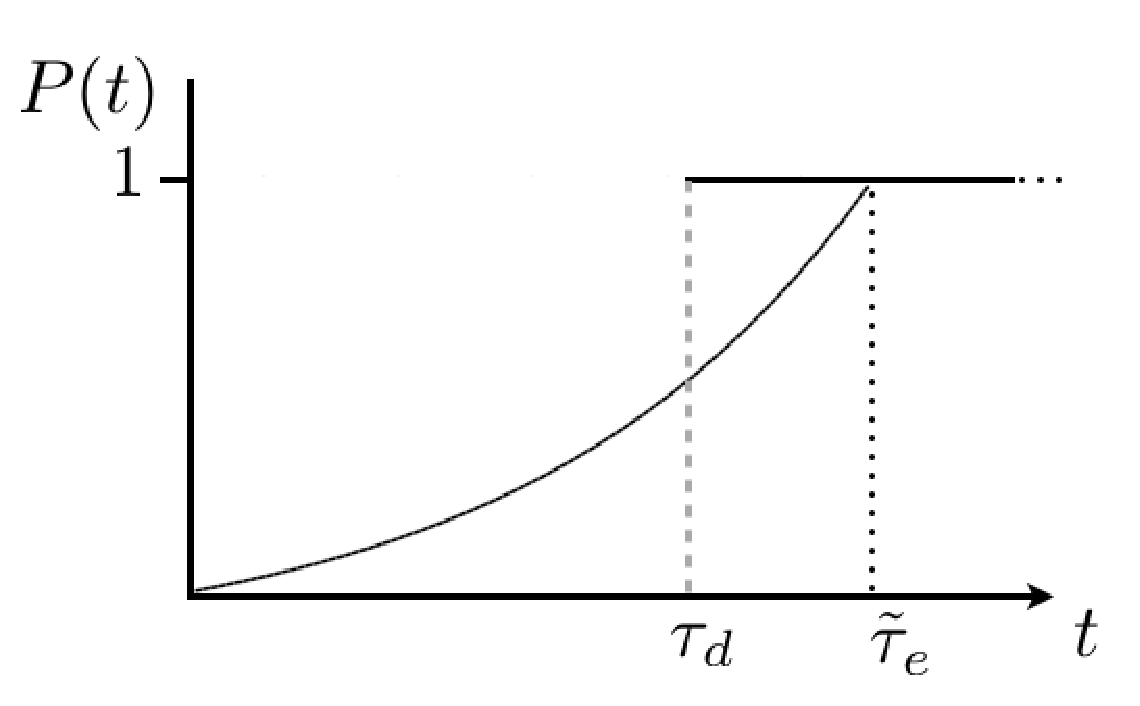
\includegraphics[width=\linewidth,angle=0]{figure5.eps}
\caption{Scheme of the emission probability procedure during the simulation. Basically are shown two different mechanism. One illustrates how works the emission probability when is imposed a dead time, the second procedure shows a exponential emission of probability.}  
\label{fig5}
\end{figure}

\begin{figure}[h]
\vspace {0.5 cm}
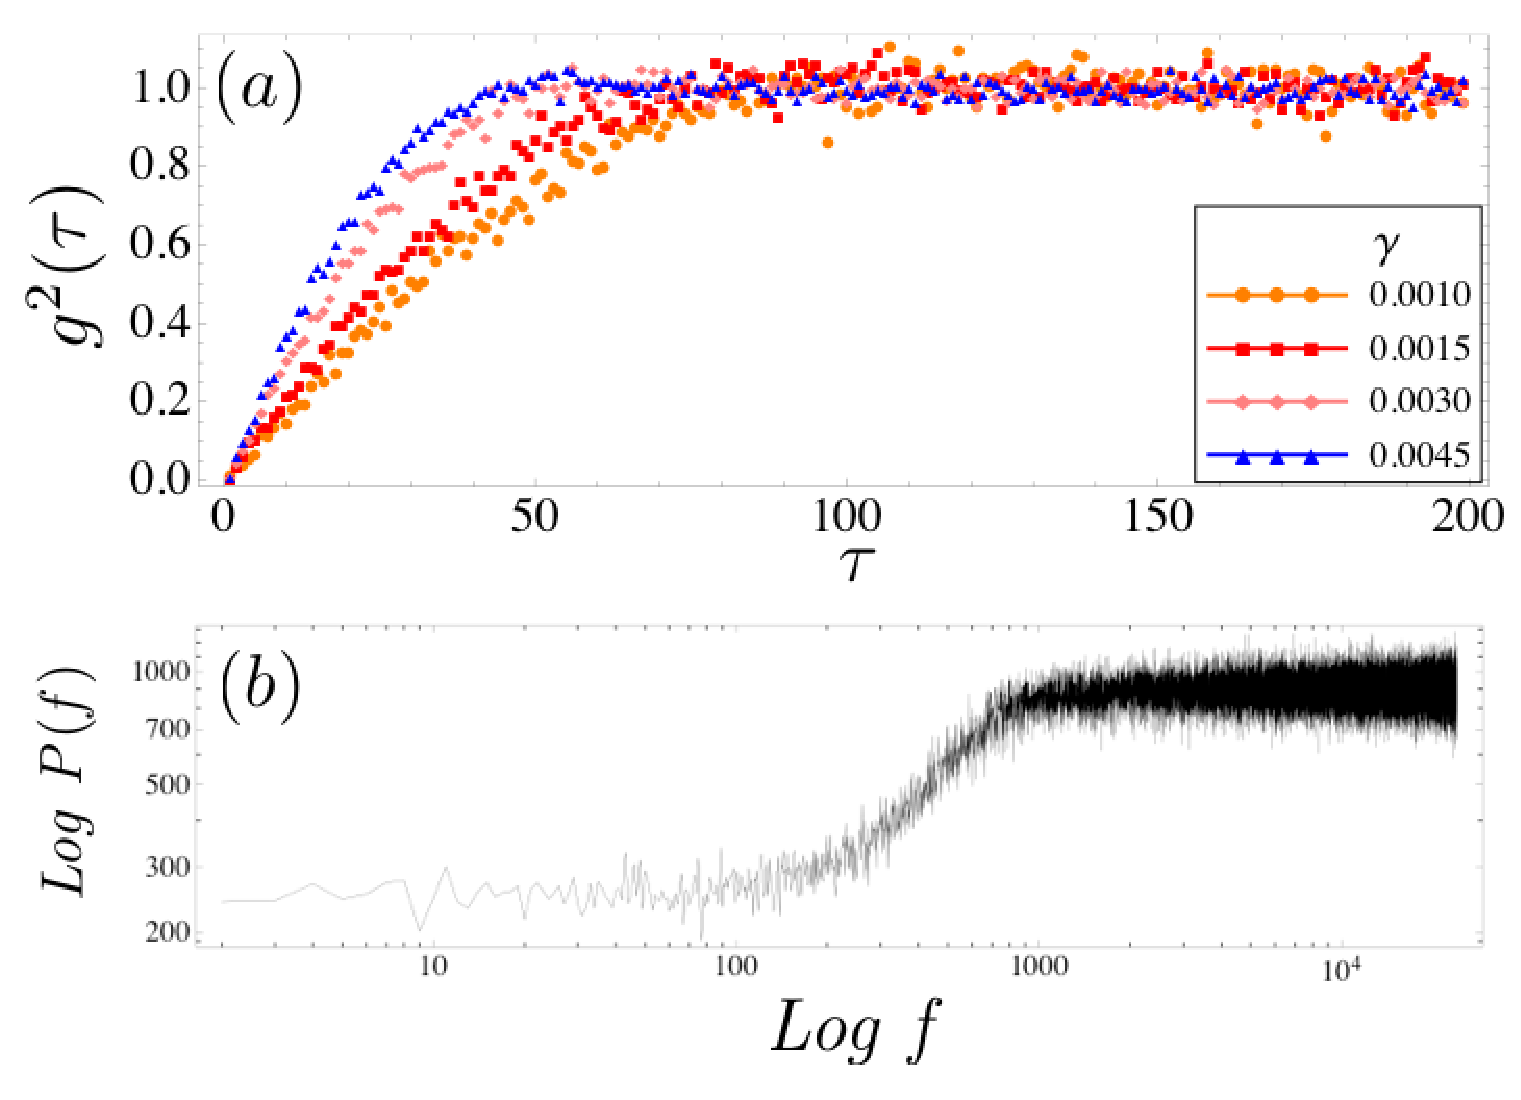
\includegraphics[width=\linewidth,angle=0]{figure6.eps}
\caption{(a) $g^{2}(\tau)$ as a function of lag time values $\tau$ to obtain the coincidence rate for time series obtained through exponential deletion control to introduce anticorrelations into the uncorrelated time series. (b) $P(f)$ obtained from a time series generated with exponential time deletion with $\gamma =0.0030$, the same behavior was found for the other values of $\gamma$.}  
\label{fig6}
\end{figure}

\begin{figure}[h]
\vspace {0.5 cm}
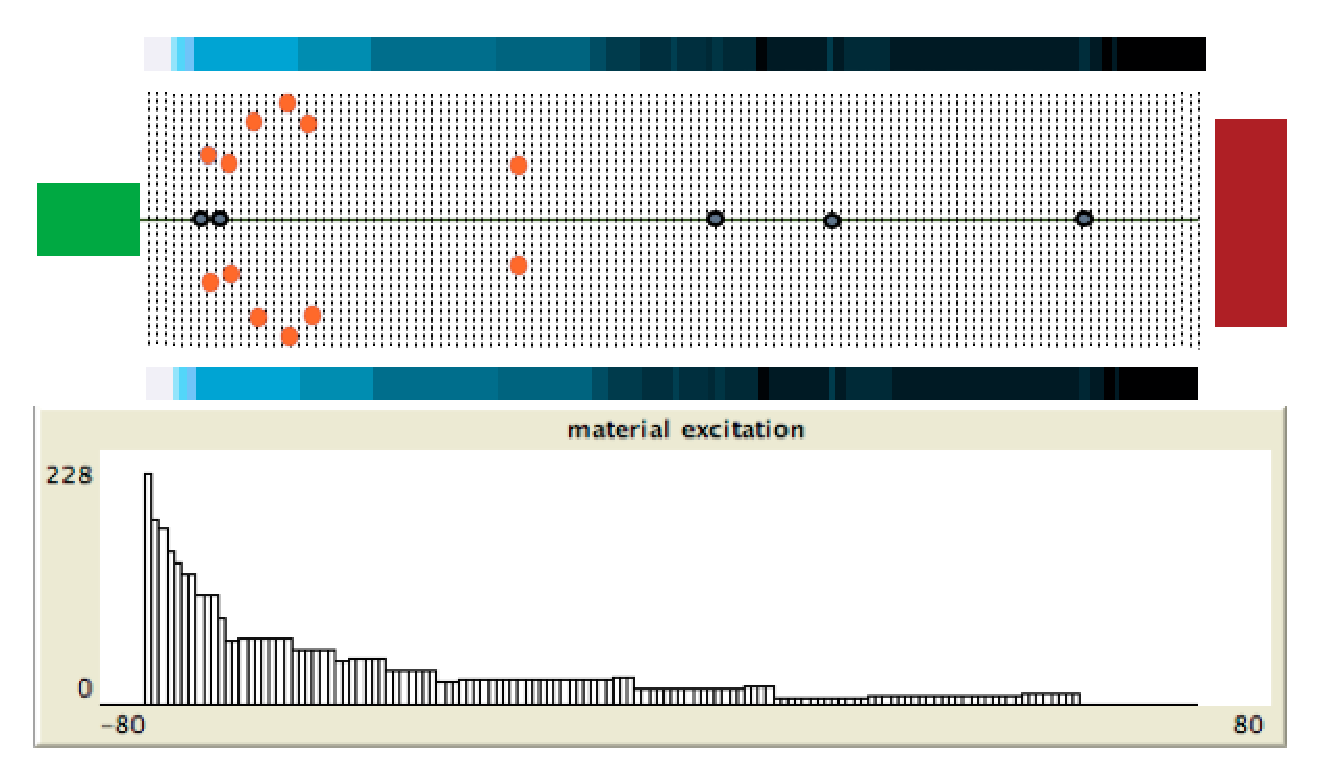
\includegraphics[width=\linewidth,angle=0]{figure7.eps}
\caption{(Color online) A hypothetical gun (green block) generates a stream of balls that have a Poisson number distribution. The slices of the medium are represented by dashed lines in the upper panel. We place a detector (red block) at the end in charge to measure. The excitation of the material can be seen in the bars placed above and below of the slices as a degradation of white to black colour through smooth green, for instance close to the gun $\xi_{e}$ takes the most high excitation (white colour). The excitation rate variation can be seen also in the lower panel with a graphic. The red small balls were converted due the nature imposed by the medium and are outside the straight path of our interest. The length of the material during the simulations is $\acute{x}=150$.}  
\label{fig7}
\end{figure}

\begin{figure}[h]
\vspace {0.5 cm}
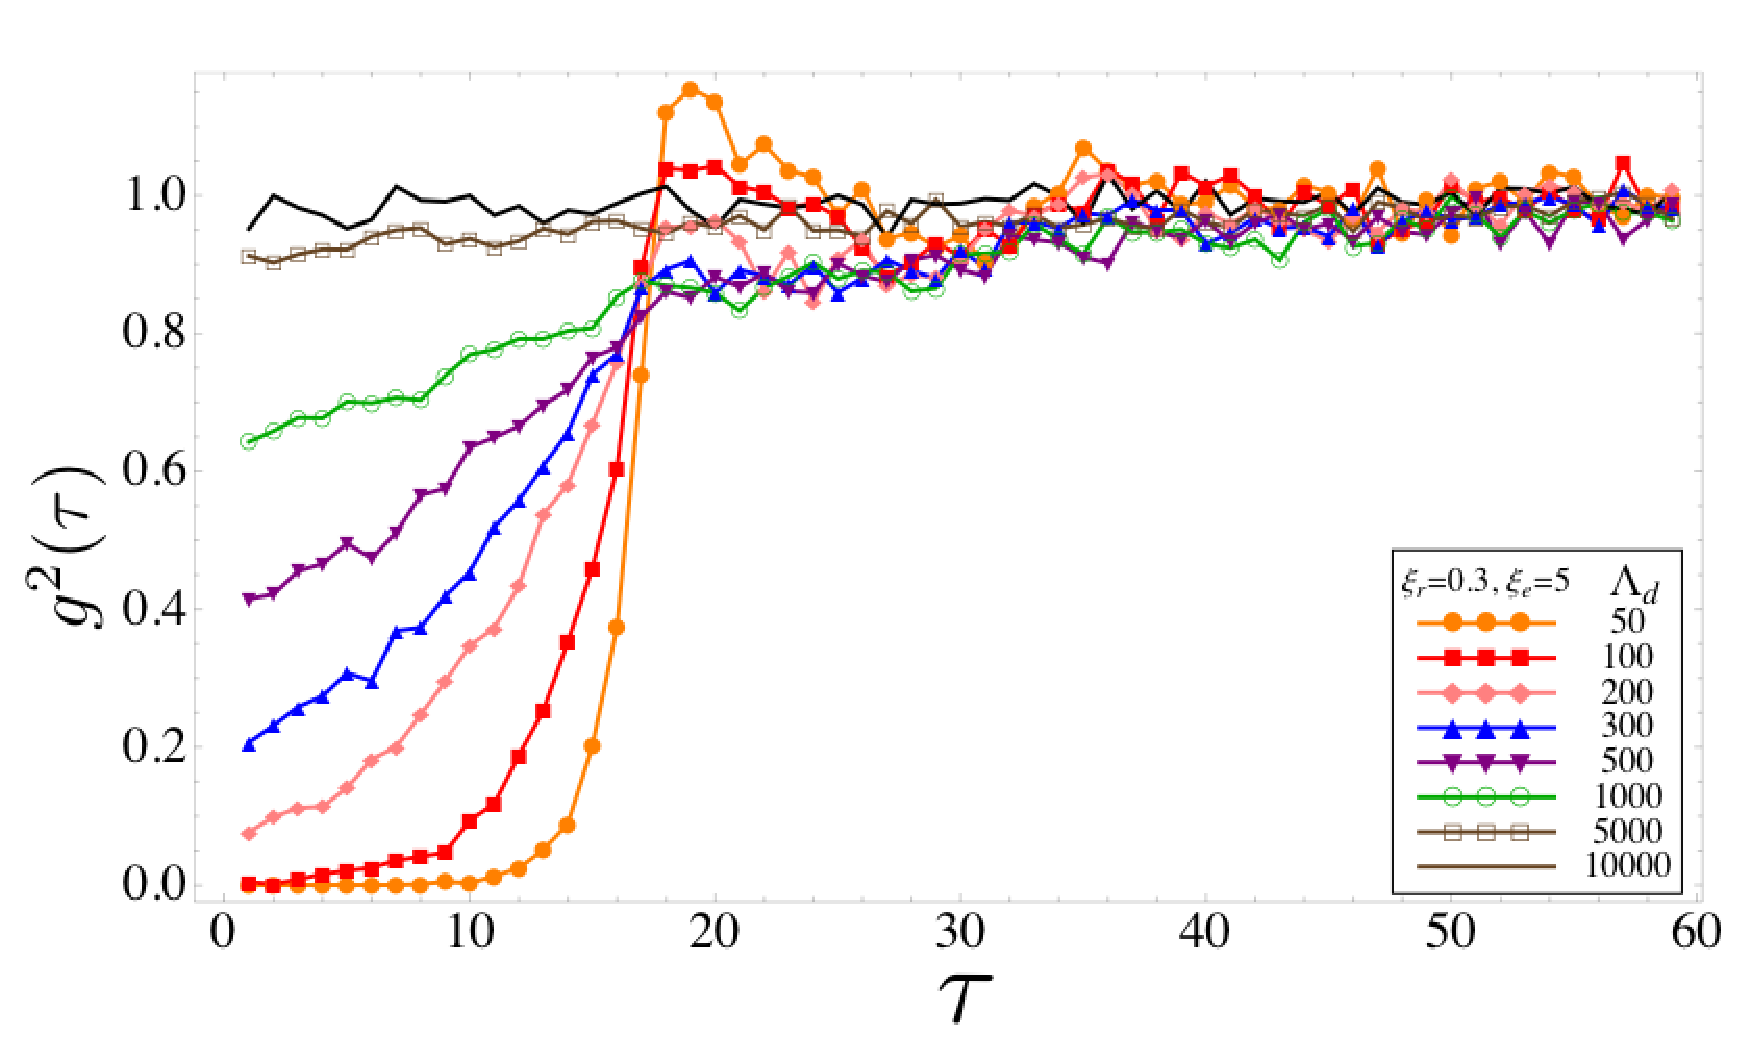
\includegraphics[width=\linewidth,angle=0]{figure8.eps}
\caption{The normalized coincidence rate $g^{2}(\tau)$ as a function of lag time values $\tau$ for different values $\Lambda_{d}$ with $\xi_{e}$ and $\xi_{r}$ fixed as is shown in Table~\ref{table1}. The important property noted is how the intensity value of $g^{2}(\tau)$ varies according of  $\Lambda_{d}$ parameter.}  
\label{fig8}
\end{figure}

\begin{figure}[h]
\vspace {0.5 cm}
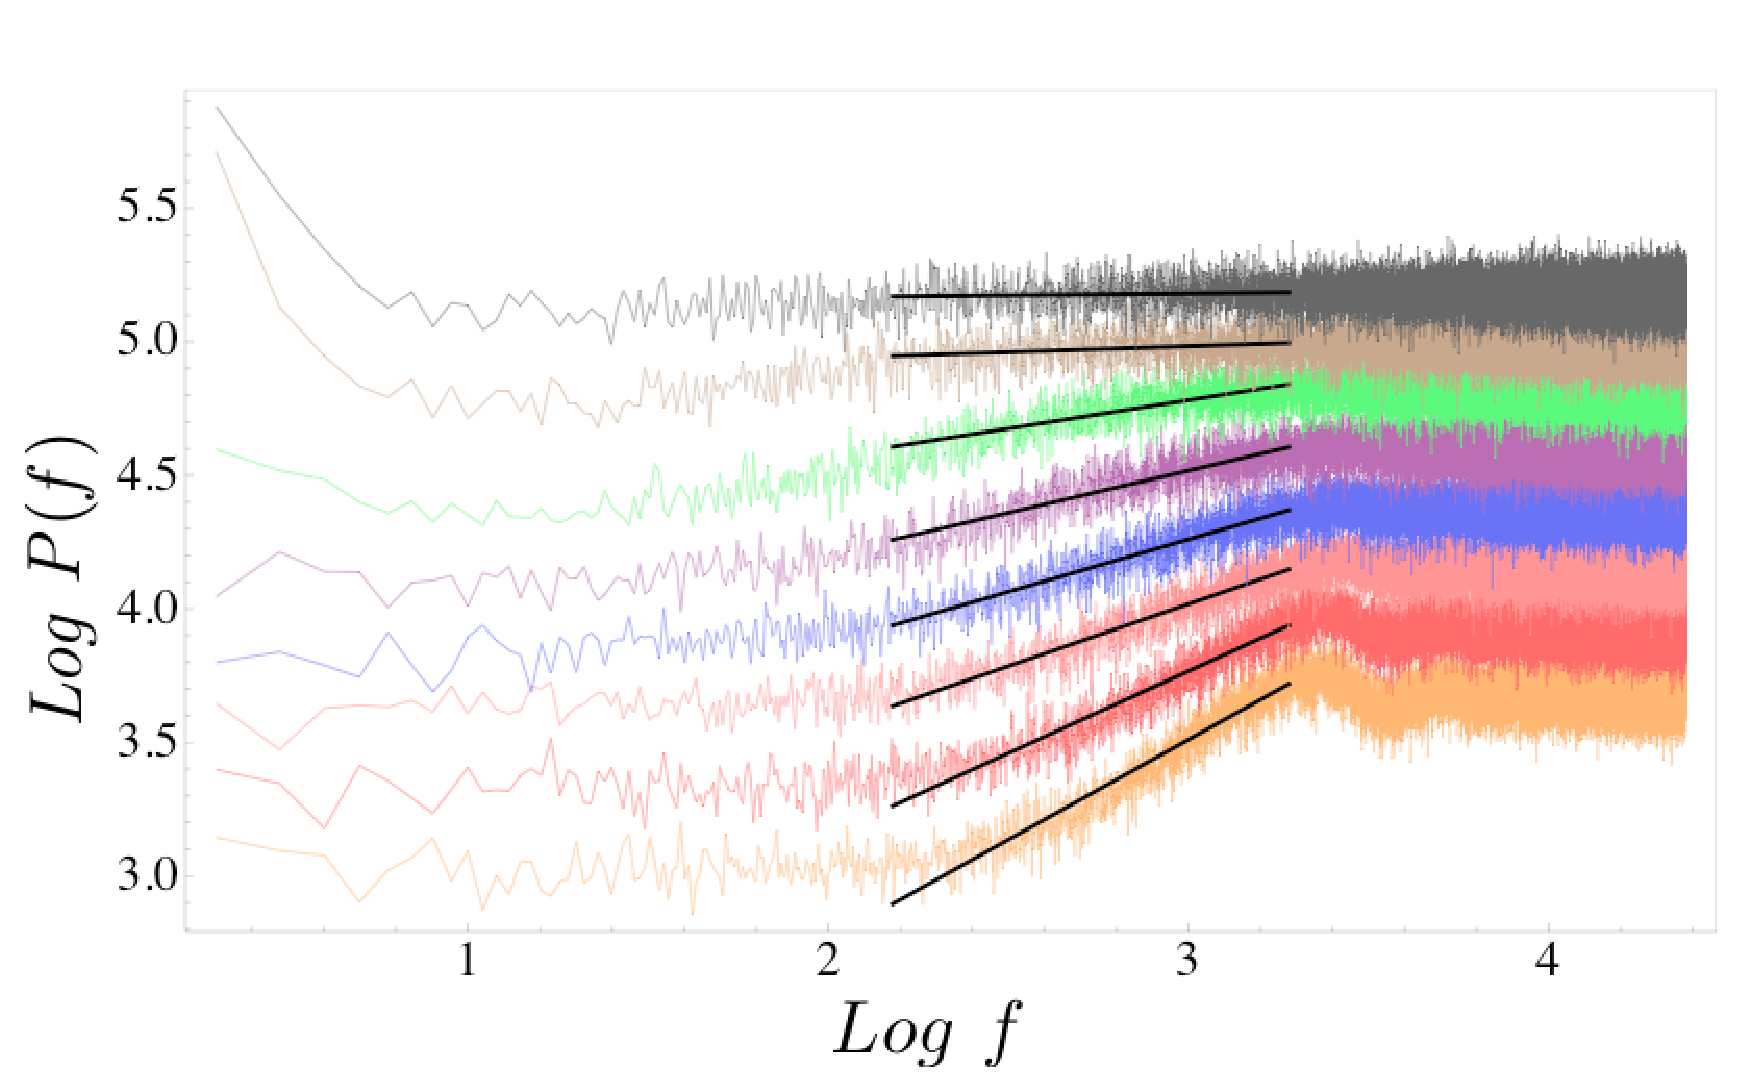
\includegraphics[width=\linewidth,angle=0]{figure9.eps}
\caption{Power spectra to the photon time series generated through a nonlinear crystal is presented. Each one corresponds to one value of $\Lambda_{d}$ with the others parametros fixed as can seen in the Table~\ref{table1}. A linear fit is shown in the plots with a thick black line only for the relevant part in the frequency domain. For the two last upper power spectrum, the linear trend extends indicating an equal contribution of the frequencies and random photon number statistics of the photon time series. Each plot was moved along the vertical axis to avoid overlapping.}  
\label{fig9}
\end{figure}

\begin{figure}[h]
\vspace {0.5 cm}
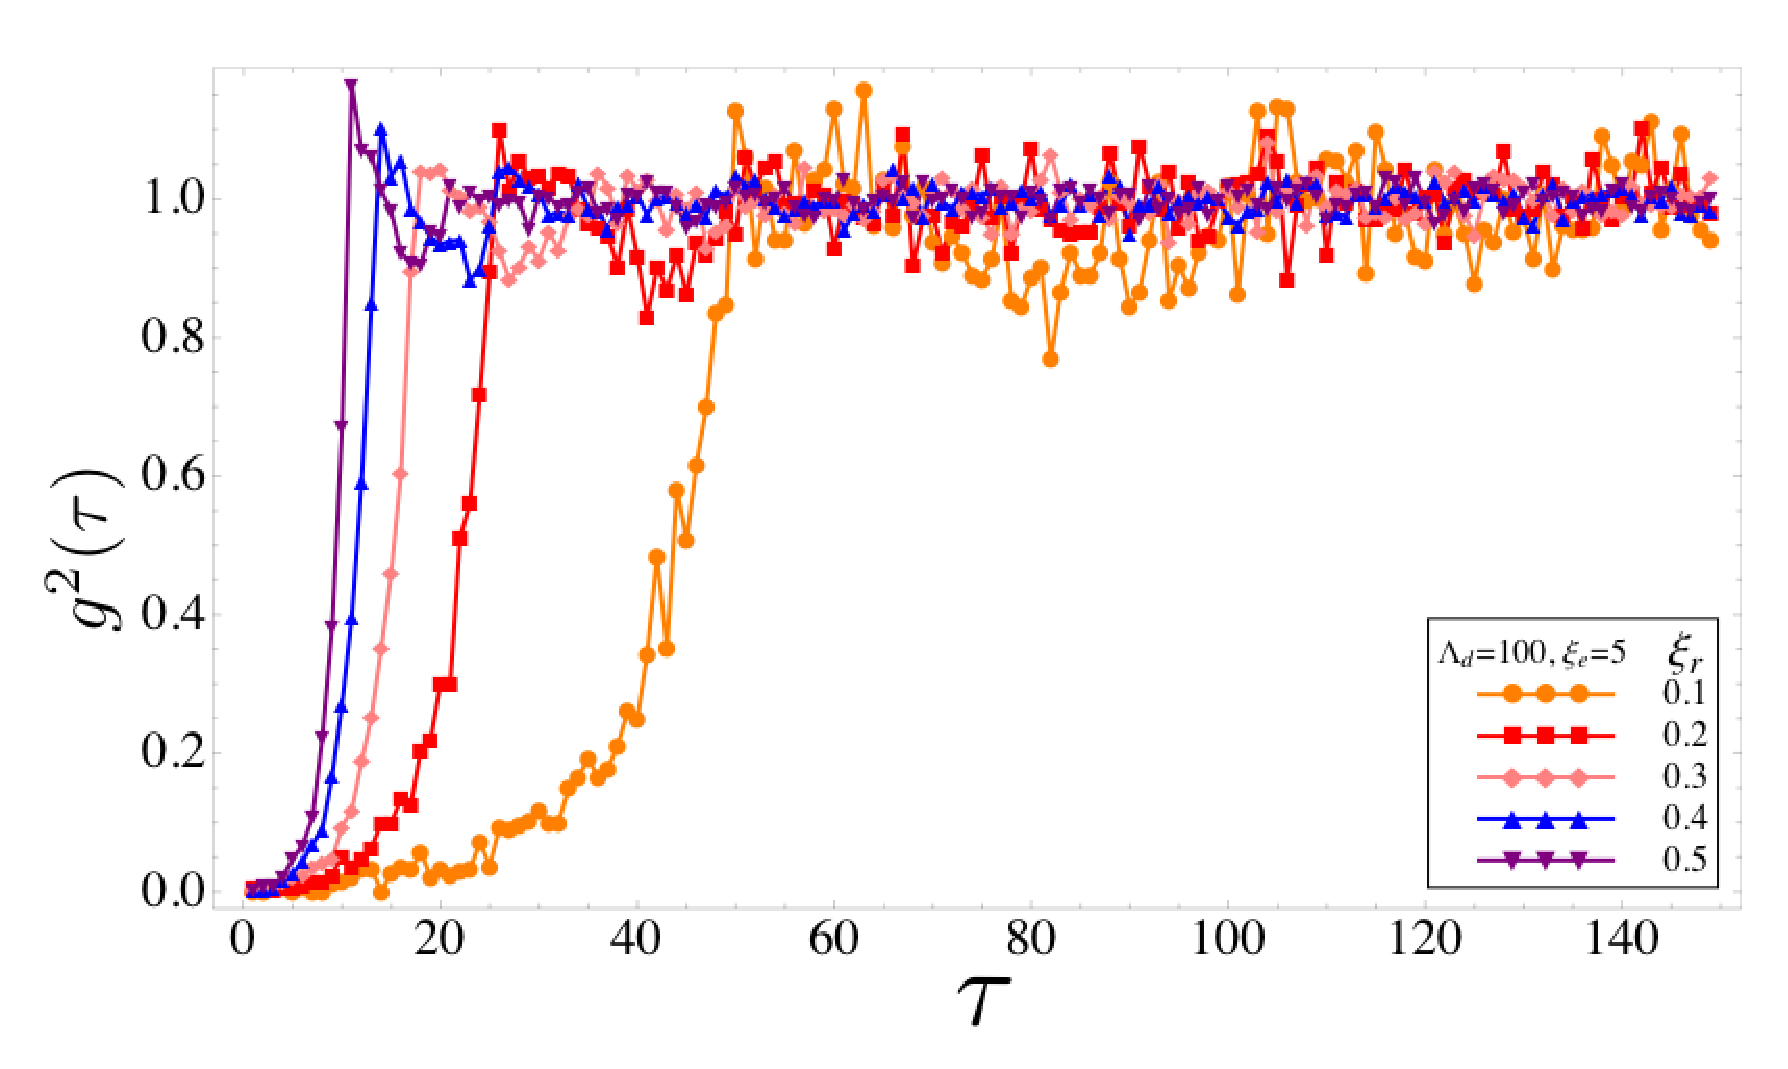
\includegraphics[width=\linewidth,angle=0]{figure10.eps}
\caption{$g^{2}(\tau)$ as a function of lag time values $\tau$ for different values $\xi_{r}$ with $\Lambda_{d}$ and $\xi_{e}$ fixed. An important property can be observed is the lon range of $g^{2}(\tau)$ is changing according the value of $\Lambda_{d}$ parameter.}  
\label{fig10}
\end{figure}

\begin{figure}[h]
\vspace {0.5 cm}
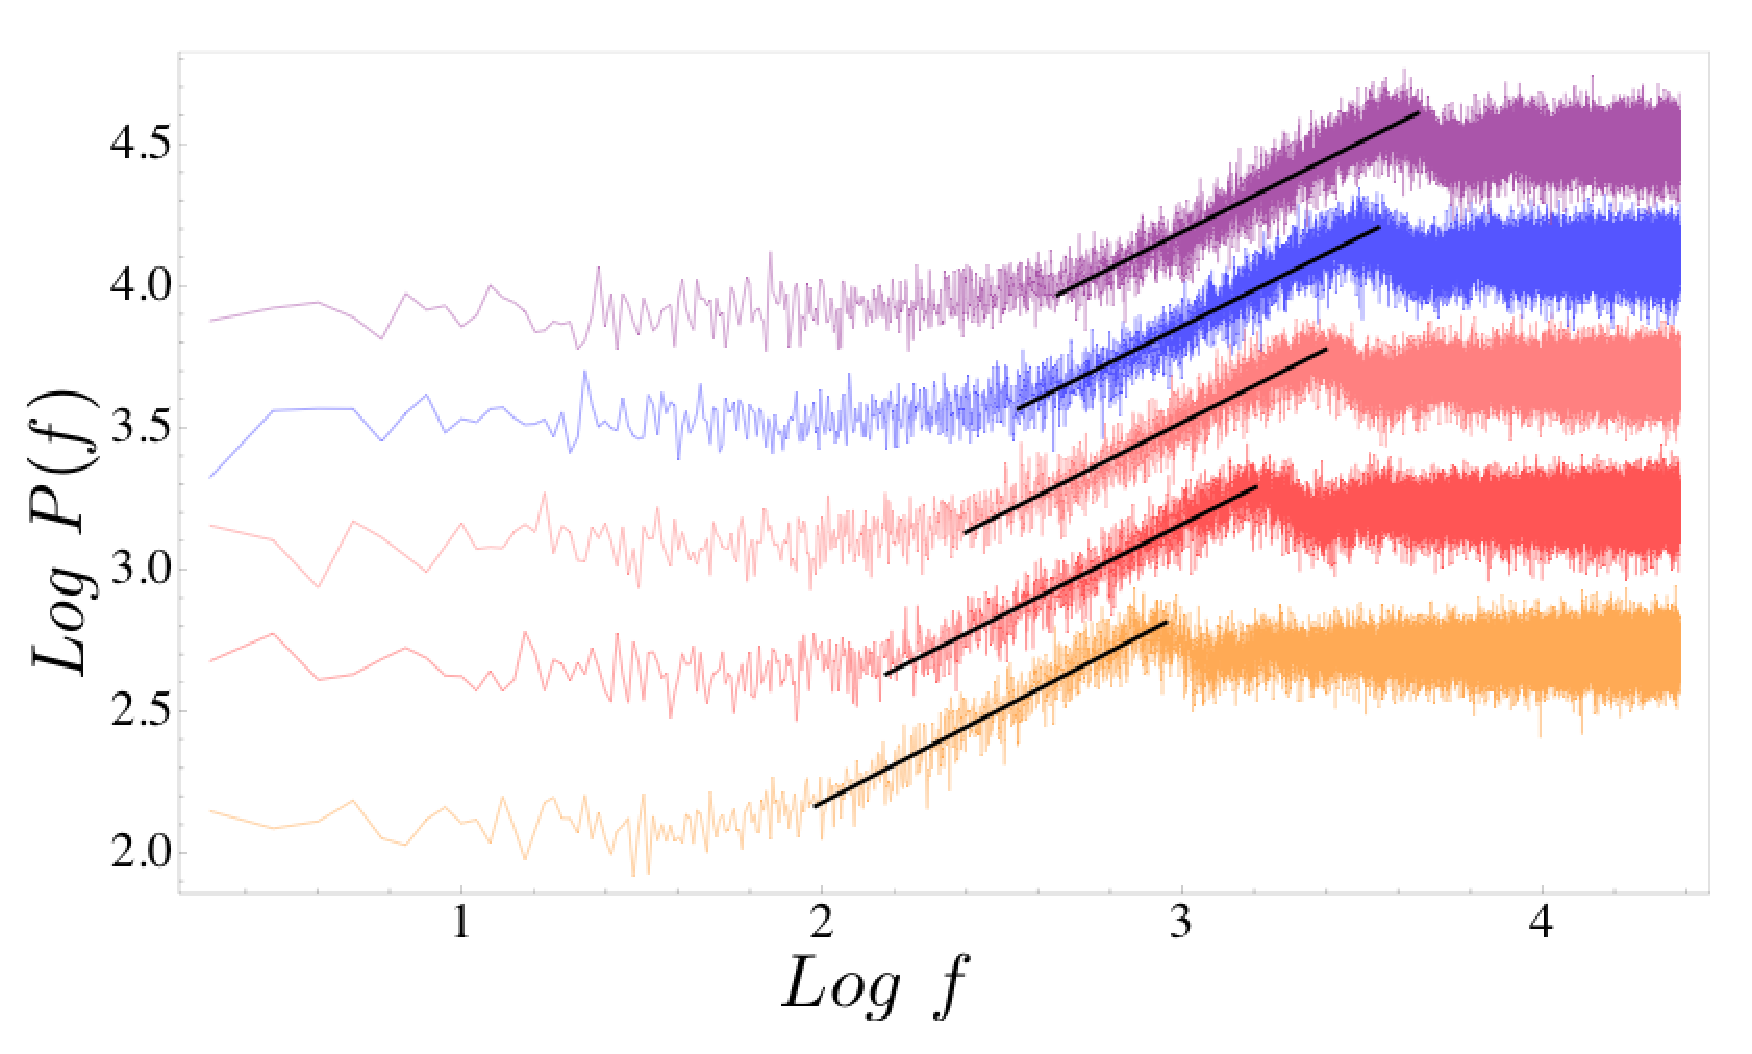
\includegraphics[width=\linewidth,angle=0]{figure11.eps}
\caption{Power spectrum $P(f)$ for the corresponding time series generated through a non linear crystal where the parameter $\xi_{r}$ is changing as can be seen in the figure legend. A linear fit is show in the plots with a thick black line just for the liner trend in the spectrum and only in the frequency domain that is interest for us and is clear a shift in the domain for different values of $\xi_{r}$. Each plot was moved along the vertical axis to avoid overlapping.}  
\label{fig11}
\end{figure}

\begin{table}
   \caption{Fano factor and the exponent $\beta_{\mathrm {ps}}$ for the time series with different values ??of the parameter $\Lambda_{d}$ \& $\xi_{e}=5$, $\xi_{r}=0.3$.}
%\begin{center}
    \begin{tabular}{@{\vrule height 10.5pt depth4pt  width0pt} | l | c | c | c | c | c | c | c | c | r |}
    \hline
\multicolumn{9}{|c|}{Fano factor ($F_{\mathrm {ps}}$) \& $\beta_{PS}$, $\xi_{e}=5$, $\xi_{r}=0.3$} \\
\hline
    \hline 
     $\Lambda_{d}$& 50 & 100 & 200 & 300 & 500 &1000 &5000 & 10000 
     \\ \hline
     $F_{\mathrm {ps}}$  & 0.24 & 0.27 & 0.30 & 0.31 & 0.35 & 0.41 & 0.95 & 1.04  \\ \hline
     $\beta_{\mathrm {ps}}$  & 0.97 & 0.66 & 0.46 & 0.39 & 0.32 & 0.21 & 0.05 & 0.01   \\ \hline
    \end{tabular}
\label{table1}
%\end{center}
\end{table}

\end{document}

